%!TEX root = ../dissertation.tex
\chapter{Aperture effects in Stellar Mass Estimates}

\label{ch:acm}
\newpage

\section{Introduction}

In this chapter we investigate methods of constraining the star formation histories and stellar masses of galaxies where galaxy spectra is available. In particular, we look at the largest galaxy catalogue of estimated stellar masses, star formation rates and gas metallicities (the MPH-JHU catalogue) obtained for the Sloan Digital Sky Survey (SDSS) Legacy Survey. The MPA-JHU catalogue has, over the last decade and a half, been one of the most influential and widely-used catalogues, both in the fields of galaxy formation and evolution as well as cosmology.\\
The SDSS spectra are obtained for multiple objects at a given time. This is done by connecting the spectrographs to fiber optic cables which are plugged into an aluminum plate that is placed in the telescope?s focal plane. These optical fibers have a fiber diameter of $3$". Thus for each galaxy in the SDSS, while photometry is available for the entire galaxy, spectra are available only for the region of the galaxy contained within this $3$" transverse angular distance and thus the fraction of the galaxy falling within the aperture may vary widely with the redshift of this galaxy. The MPA-JHU catalogue was developed by using a sophisticated workaround this problem as described below.\\
The stellar masses in the catalogue and consequently, the star formation histories are obtained by looking at two key spectral indicators of starbursts and age of a galaxy: the Balmer $h\delta_{A}$ absorption line index and the $D_{n}4000$ break index, both of which are relatively insensitive to the metallicity-age degeneracy issue that spectral indicators in the more redder side of the spectrum are limited by. Using the distribution of the observed galaxies in the $h\delta_{A}-D_{n}4000$ plane and by employing Stellar Population Synthesis (SPS) models by Bruzual et al to model the evolution of galaxies in this plane, they are able to successfully infer a mass-to-light ratio in the z-band (Kauffmann et al) for every point in this phase space. From here, it is a short step to using the luminosity of the entire galaxy to successfully infer the stellar mass and star formation history of the galaxy.\\
However, this workaround can be problematic when the M/L ratio of the central part of a galaxy is not representative of the entire galaxy. This can be an issue where there are strong bulge-disc components such as spiral galaxies. However, with the availability of spatially resolved spectra for galaxies from IFU (Integral Field Unit) based surveys such as MaNGA, SAMI, MUSE, Califa etc, we can actually put this question to test and quantify the effect of aperture size on the SDSS stellar masses. We use MaNGA, the largest IFU-based survey thusfar and ask the following questions: At any given redshift in the local Unverse, how does the position of the galaxy in the $h\delta_{A}-D_{n}4000$ plane as measured using a $3$" aperture compare to using a full aperture, i.e. spectra from all the spatially resolved regions in the galaxy.\\


\subsection{The SDSS spectra}
Describing the SDSS spectrograph and $3$ arcsec fiber diameter. References: York et al; Smee et al.

The galaxy spectra in SDSS are obtained through $3$ arcsec diameter fibers. The rest-frame wavelength range of the spectra at median wavelength range from $3500$ to $8500$ with a spectral resolution ($R = \frac{\Delta\lambda}{\lambda}$) of ~ 2000. The spectra are calibrated using observations of F stars in each 3-degree field.

\subsection{The MPA JHU Catalog}
Introduction to and describing the importance of the largest catalogue of galaxy stellar masses (Kauffmann), star formation rates (Brinchmann) and gas metallicities (Tremonti) thusfar. Including major results that rely on said SFR's.

\begin{figure}
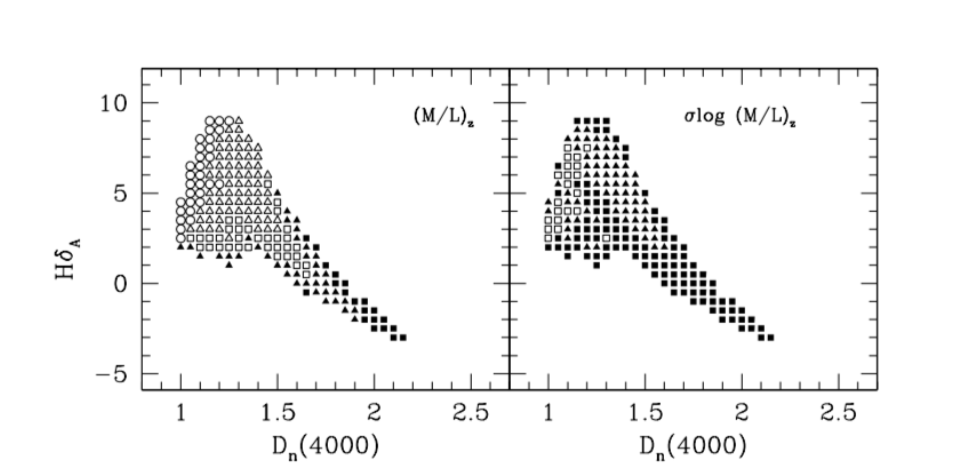
\includegraphics[width=\textwidth]{figures/Kauffmann_grid}
\caption[Short figure name.]{The Kauffmann et al grid to infer M/L ratios from the $h\delta_{A}-D_{n}4000$ plane
\label{fig:myInlineFigure}}
\end{figure}

\section{The $h\delta_{A}-D_{n}4000$ plane}

Two powerful spectral diagnostic tools that are valuable in constraining stellar masses and star formation histories in galaxies are the Balmer $\delta$ absorption line index and the $D_{n}4000$ break index in the optical spectrum of a galaxy (cite Kauffmann et. al.). One of the key issues in spectral indicators for starbursts is the existence of the age-metallicity degeneracy in stellar populations. (cite Worthey et. al.) The heavier element lines are often prominent in both early type as well as metal rich galaxies and the two are hard to distinguish in terms of interpretation as older stellar populations exhibit metal richness as well and without accurate modeling of the chemical evolution of galaxies, it is difficult to ascertain the reason. The Balmer $H\alpha$ and $H\beta$ are sensitive to the effects of metallicity as well. However both the Balmer $H\delta$ absorption line as well as the $D_{n}4000$ break occurring in the continuum are both in a bluer region of the spectrum relatively unaffected by metallicity constraints and together they form a powerful diagnostic tool to constrain the mass-to-light ratios of galaxies. 

\subsection{Measuring the $D_{n}4000$ index}
(Cite earliest discovery of the $D_{n}4000$ break here.)  The most obvious discontinuity in the spectrum of a galaxy is the $D_{n}4000$ break, which is a consequence of the absorption of ionized metals. In more metal rich stellar populations (i.e. older galaxies), thus, this break is large and in younger stellar populations which tend to me metal poor, this break is small. This break was defined in a broad bandpass by Bruzual et al (1983). The bandpass used in Kauffmann et al is the same as the one introduced by Balogh et al (1999) and their motivation for doing so is that the narrow definition is more insensitive to reddening effects. I reproduce these measurements using the same narrow bandpass definition.


\subsection{Measuring the $h\delta_{A}$ index}

\section{Manga Overview}
\begin{figure}
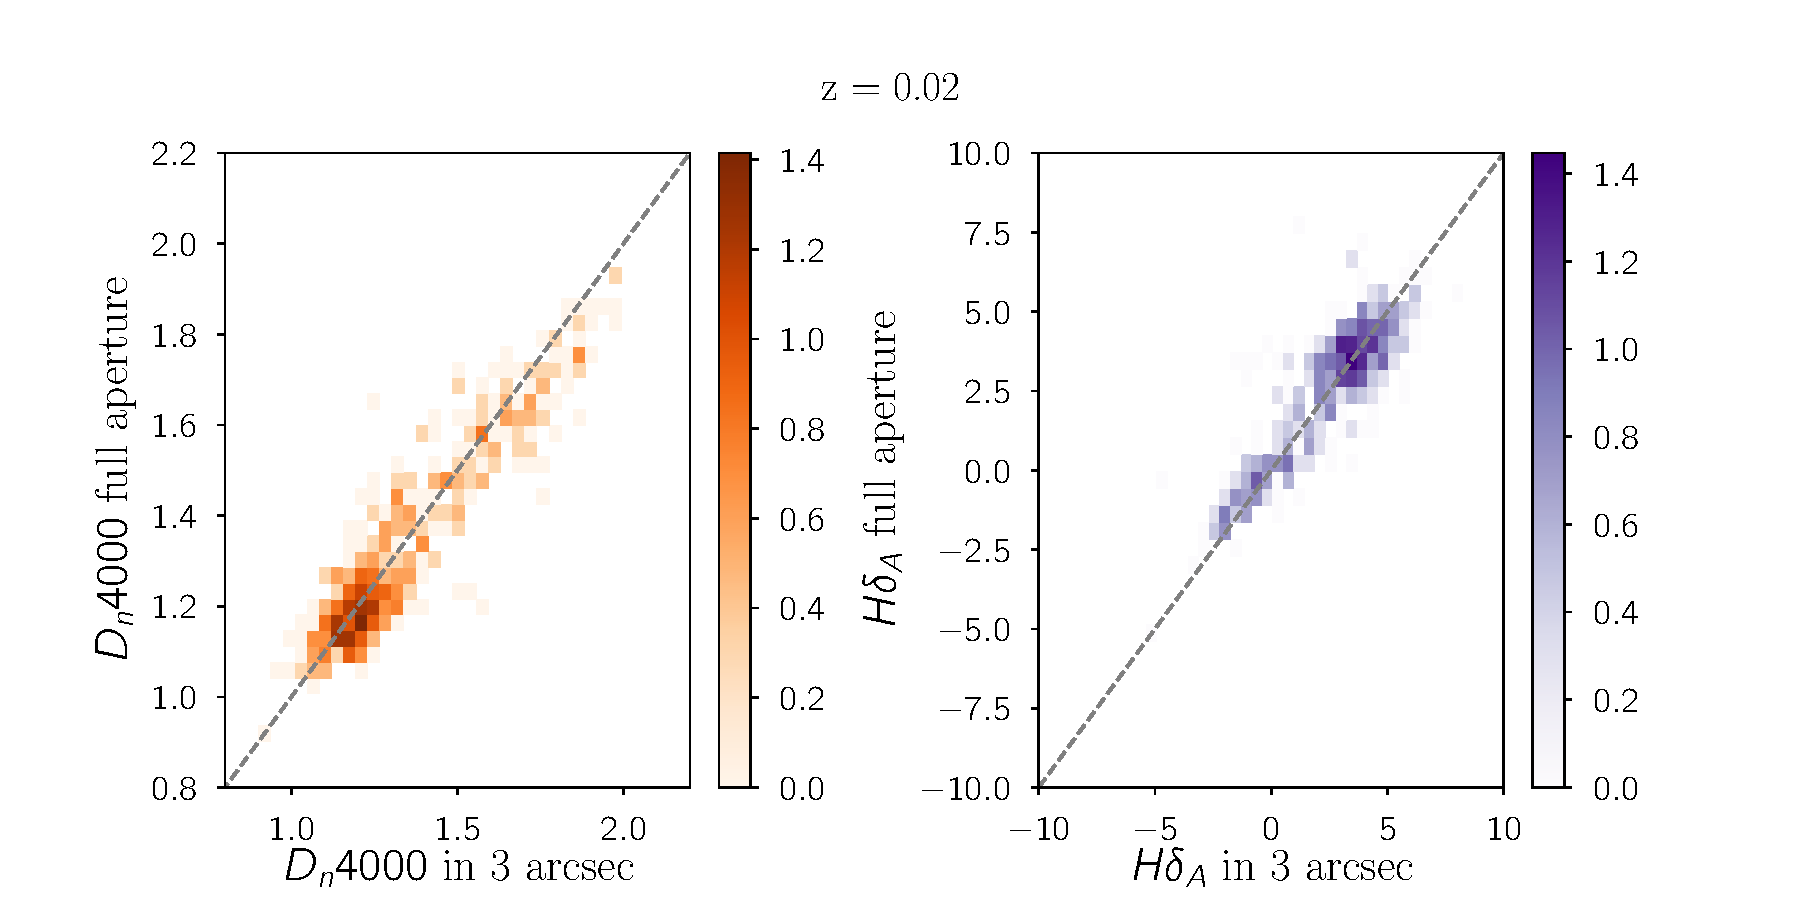
\includegraphics[width=\textwidth]{figures/a.pdf}
\caption[Short figure name.]{ The $D_{n}4000$, $h\delta_{A}$ indices measures at $z = 0.02$ with a $3$" aperture compared to the full aperture measurement
\label{fig:myInlineFigure}}
\end{figure}

\begin{figure}
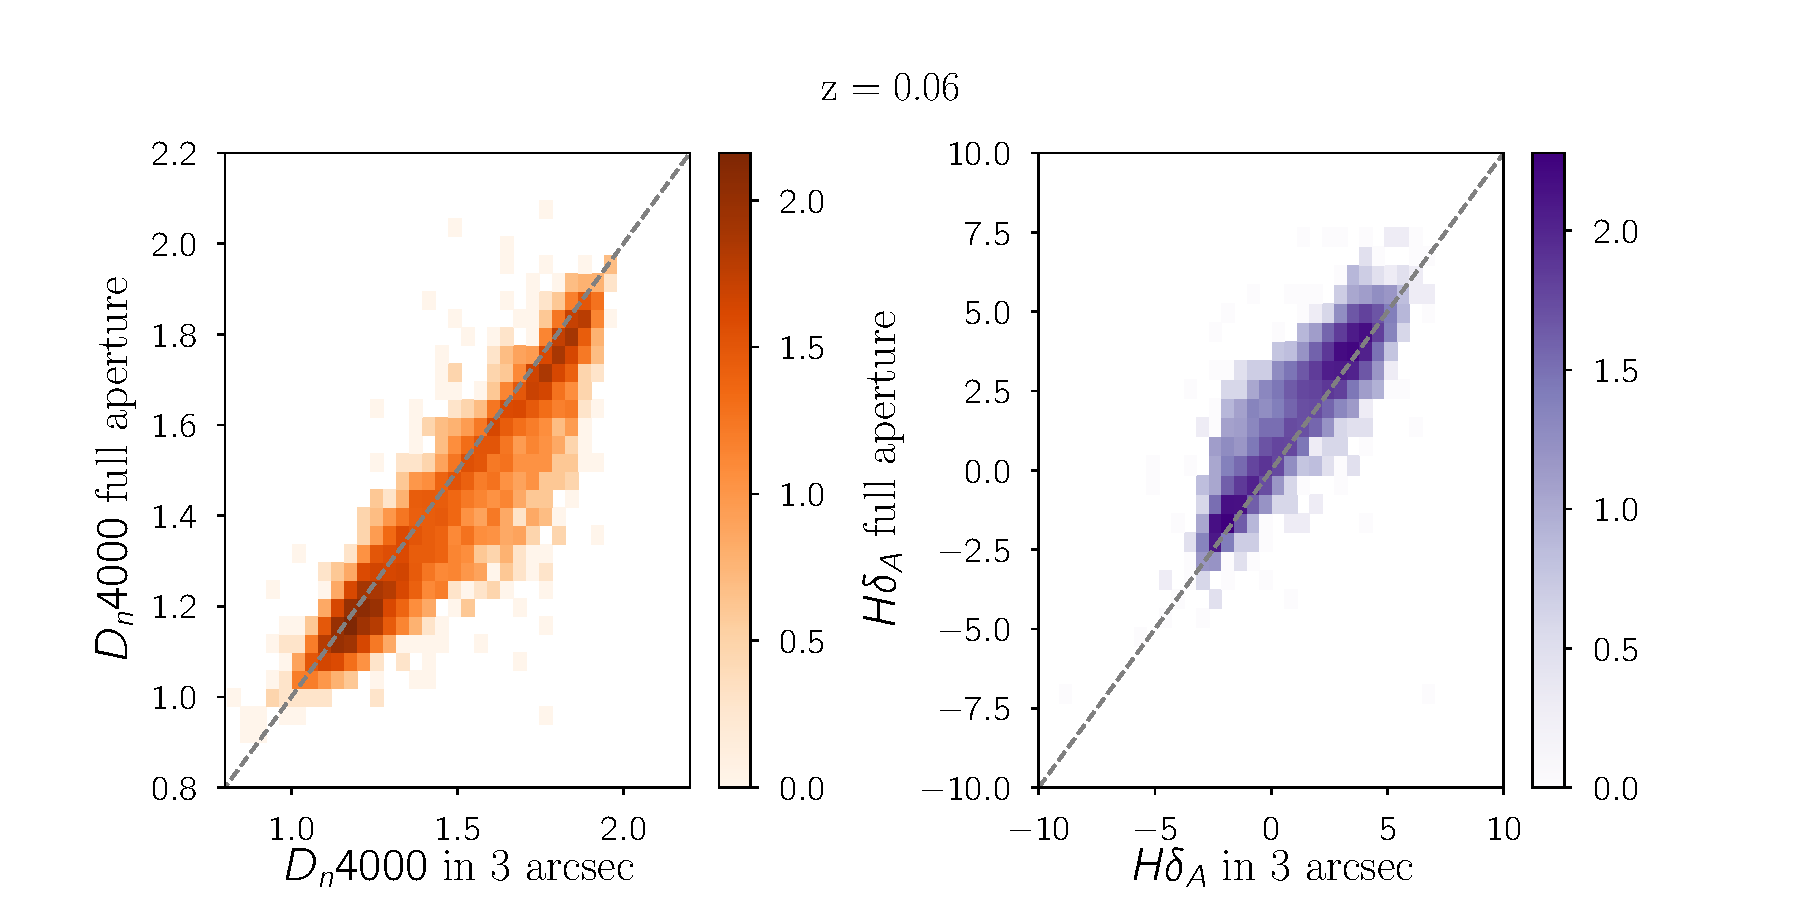
\includegraphics[width=\textwidth]{figures/b.pdf}
\caption[Short figure name.]{ The $D_{n}4000$, $h\delta_{A}$ indices measures at $z = 0.06$ with a $3$" aperture compared to the full aperture measurement
\label{fig:myInlineFigure}}
\end{figure}

\begin{figure}
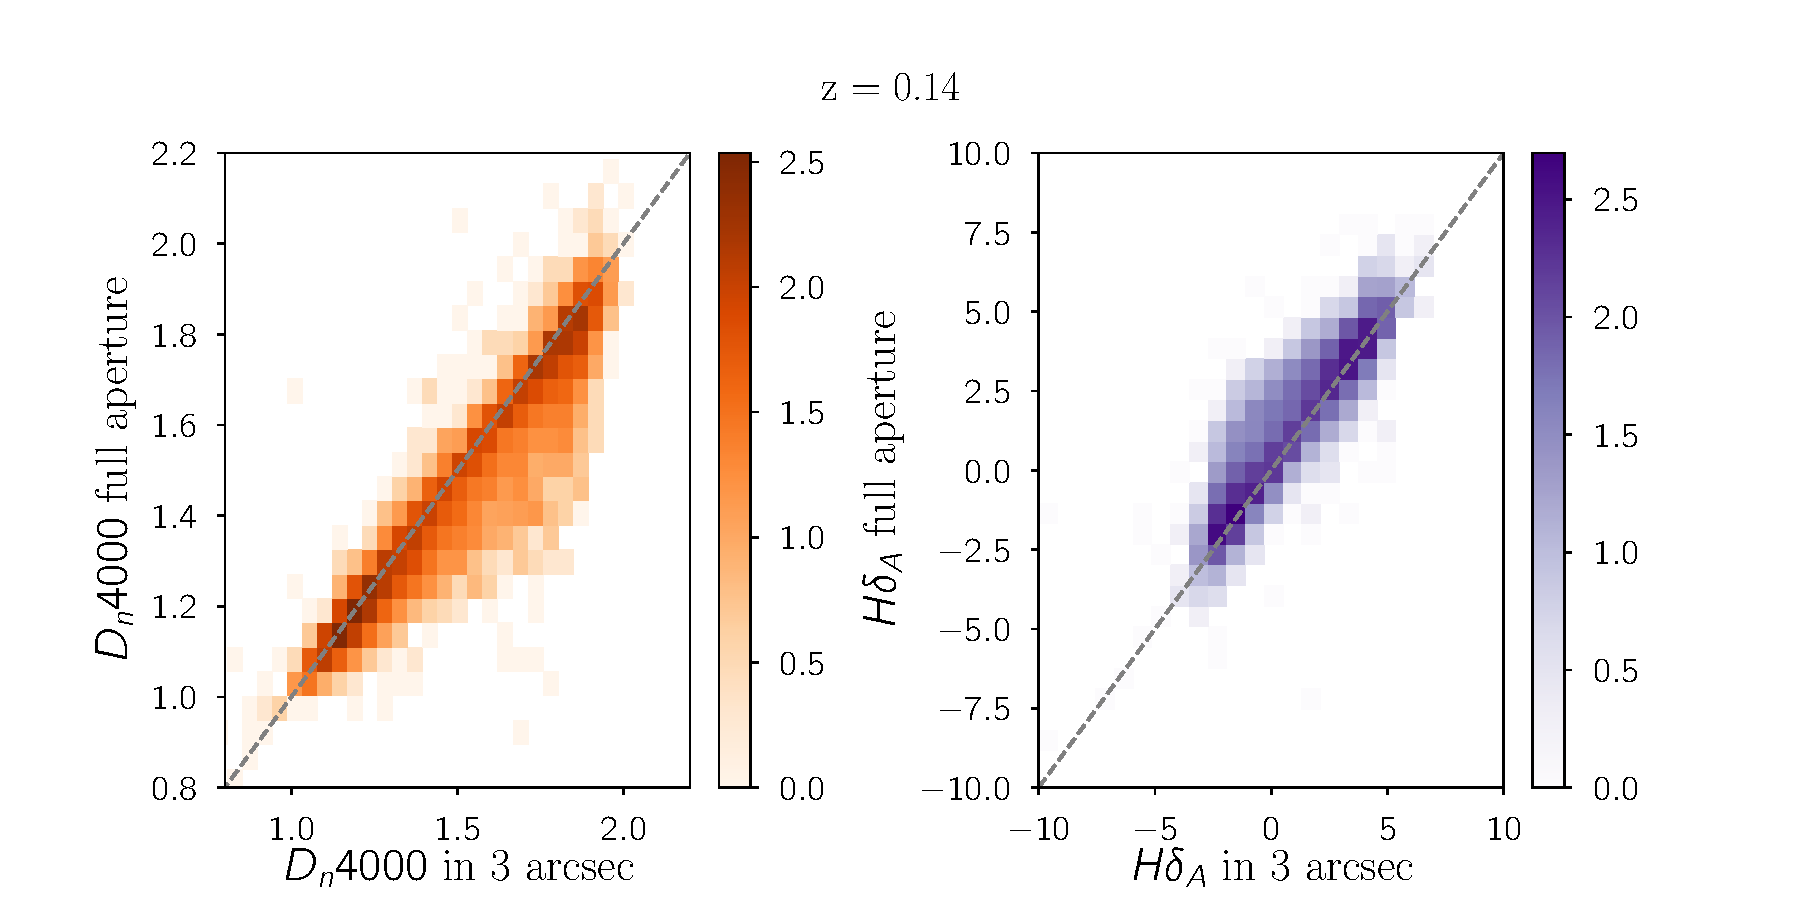
\includegraphics[width=\textwidth]{figures/c.pdf}
\caption[Short figure name.]{ The $D_{n}4000$, $h\delta_{A}$ indices measures at $z = 0.14$ with a $3$" aperture compared to the full aperture measurement
\label{fig:myInlineFigure}}
\end{figure}


\subsection{Introduction to Integral Field Spectroscopy}

\subsection{The MaNGA IFU Design}

\section{The $h\delta_{A}-D_{n}4000$ Measurements at Multiple Redshifts}
\section{Manga Overview}
\begin{figure}
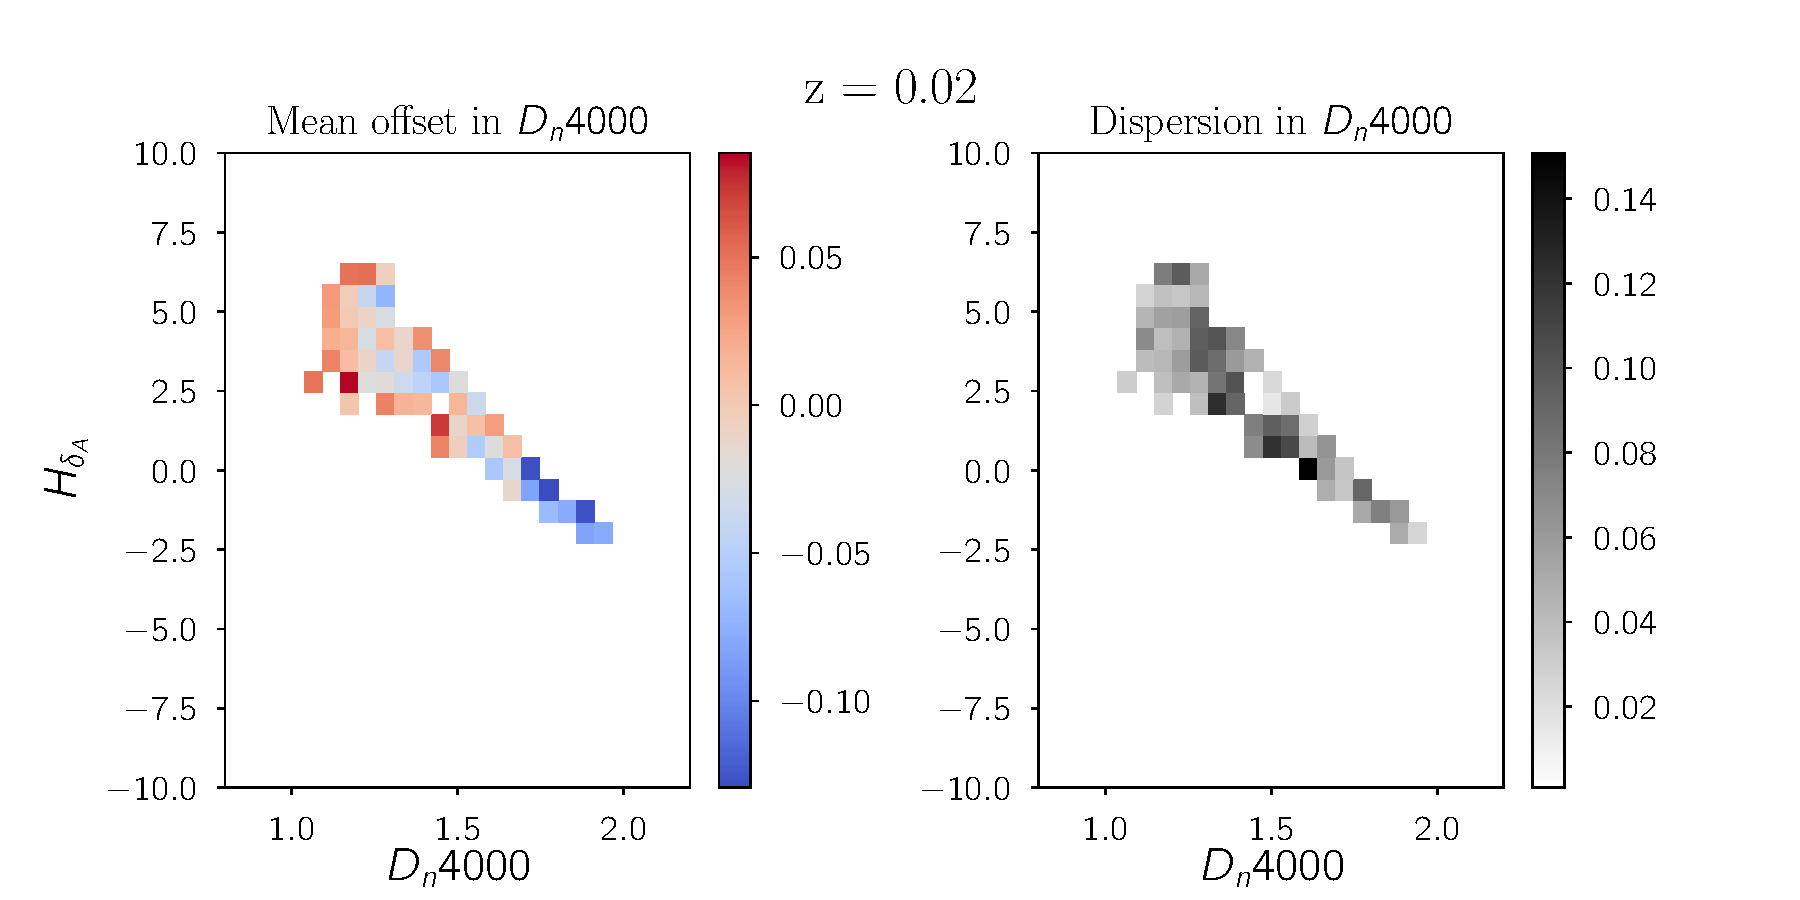
\includegraphics[width=\textwidth]{figures/zb.pdf}
\caption[Short figure name.]{ The mean offset and dispersion in the $D_{n}4000$ index measured at $z = 0.02$ with a $3$" aperture from the full aperture measurement
\label{fig:myInlineFigure}}
\end{figure}

\begin{figure}
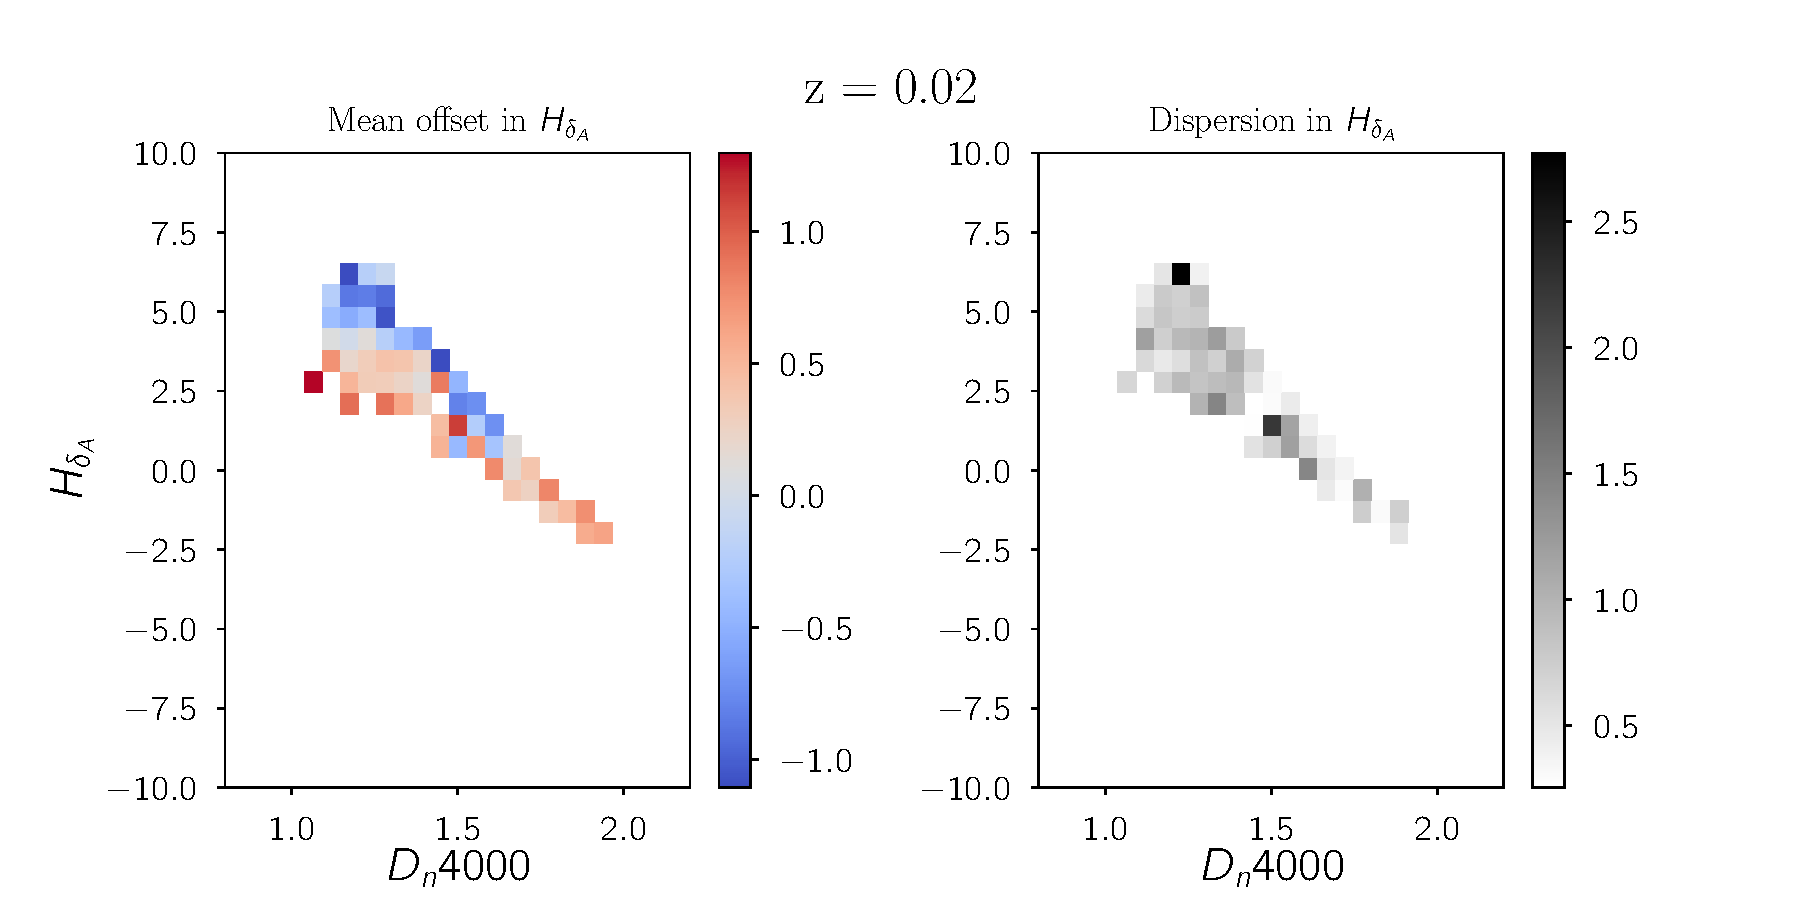
\includegraphics[width=\textwidth]{figures/zc.pdf}
\caption[Short figure name.]{ The mean offset and dispersion in the $h\delta_{A}$ index measured at $z = 0.02$ with a $3$" aperture from the full aperture measurement 
\label{fig:myInlineFigure}}
\end{figure}

\begin{figure}
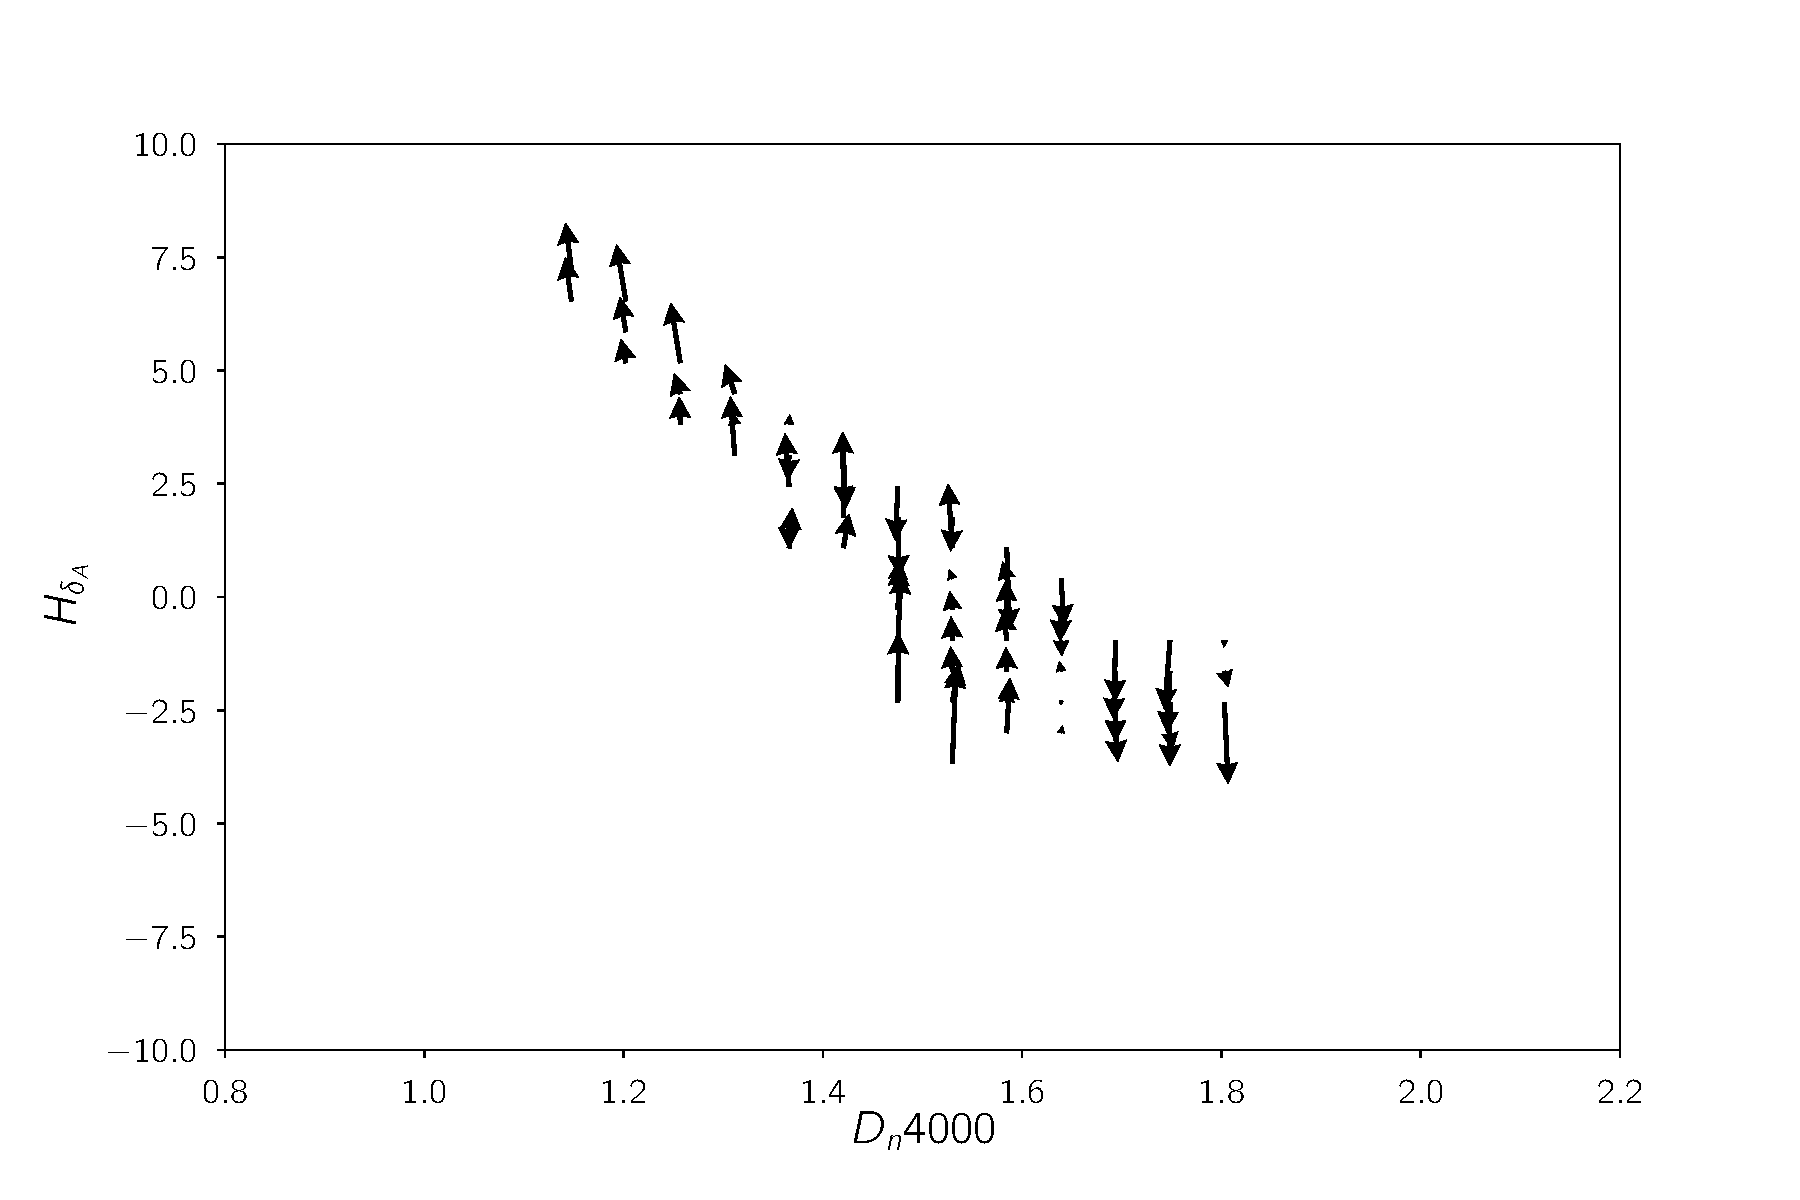
\includegraphics[width=\textwidth]{figures/zd.pdf}
\caption[Short figure name.]{ The mean offset at $z=0.02$ plotted as a vector in the $D_{n}4000$, $h\delta_{A}$ plane
\label{fig:myInlineFigure}}
\end{figure}

\section{Results}

\section{The $h\delta_{A}-D_{n}4000$ Measurements at Multiple Redshifts}
\section{Manga Overview}
\begin{figure}
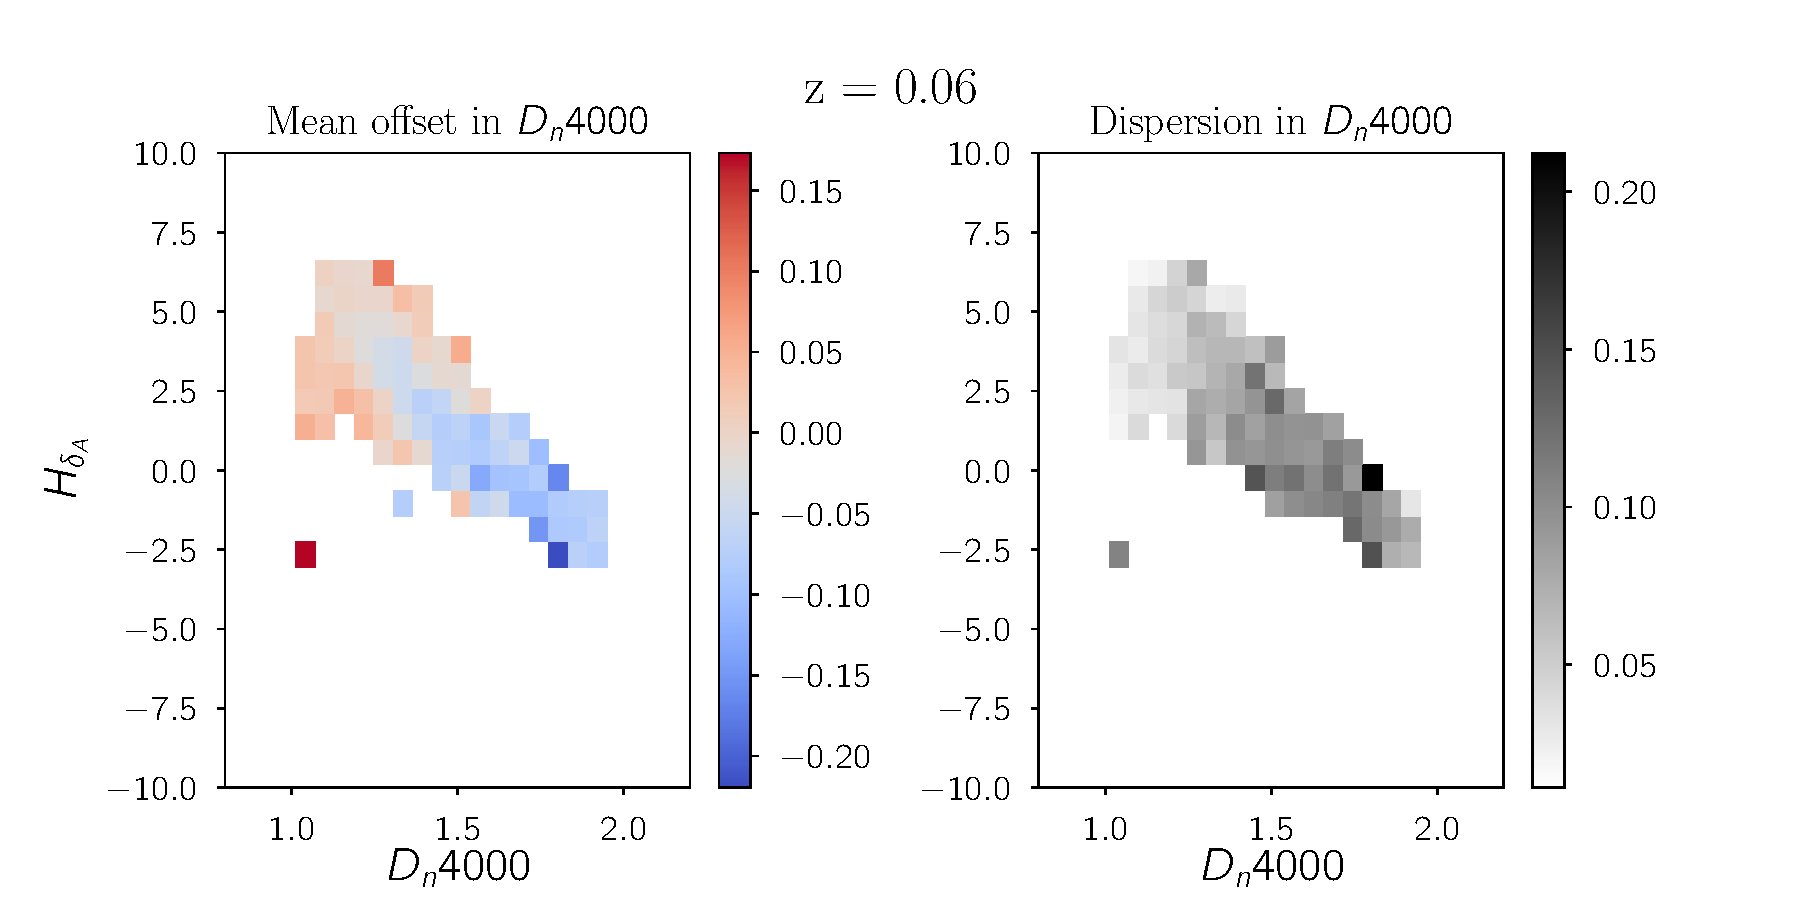
\includegraphics[width=\textwidth]{figures/z6b.pdf}
\caption[Short figure name.]{ The mean offset and dispersion in the $D_{n}4000$ index measured at $z = 0.06$ with a $3$" aperture from the full aperture measurement
\label{fig:myInlineFigure}}
\end{figure}

\begin{figure}
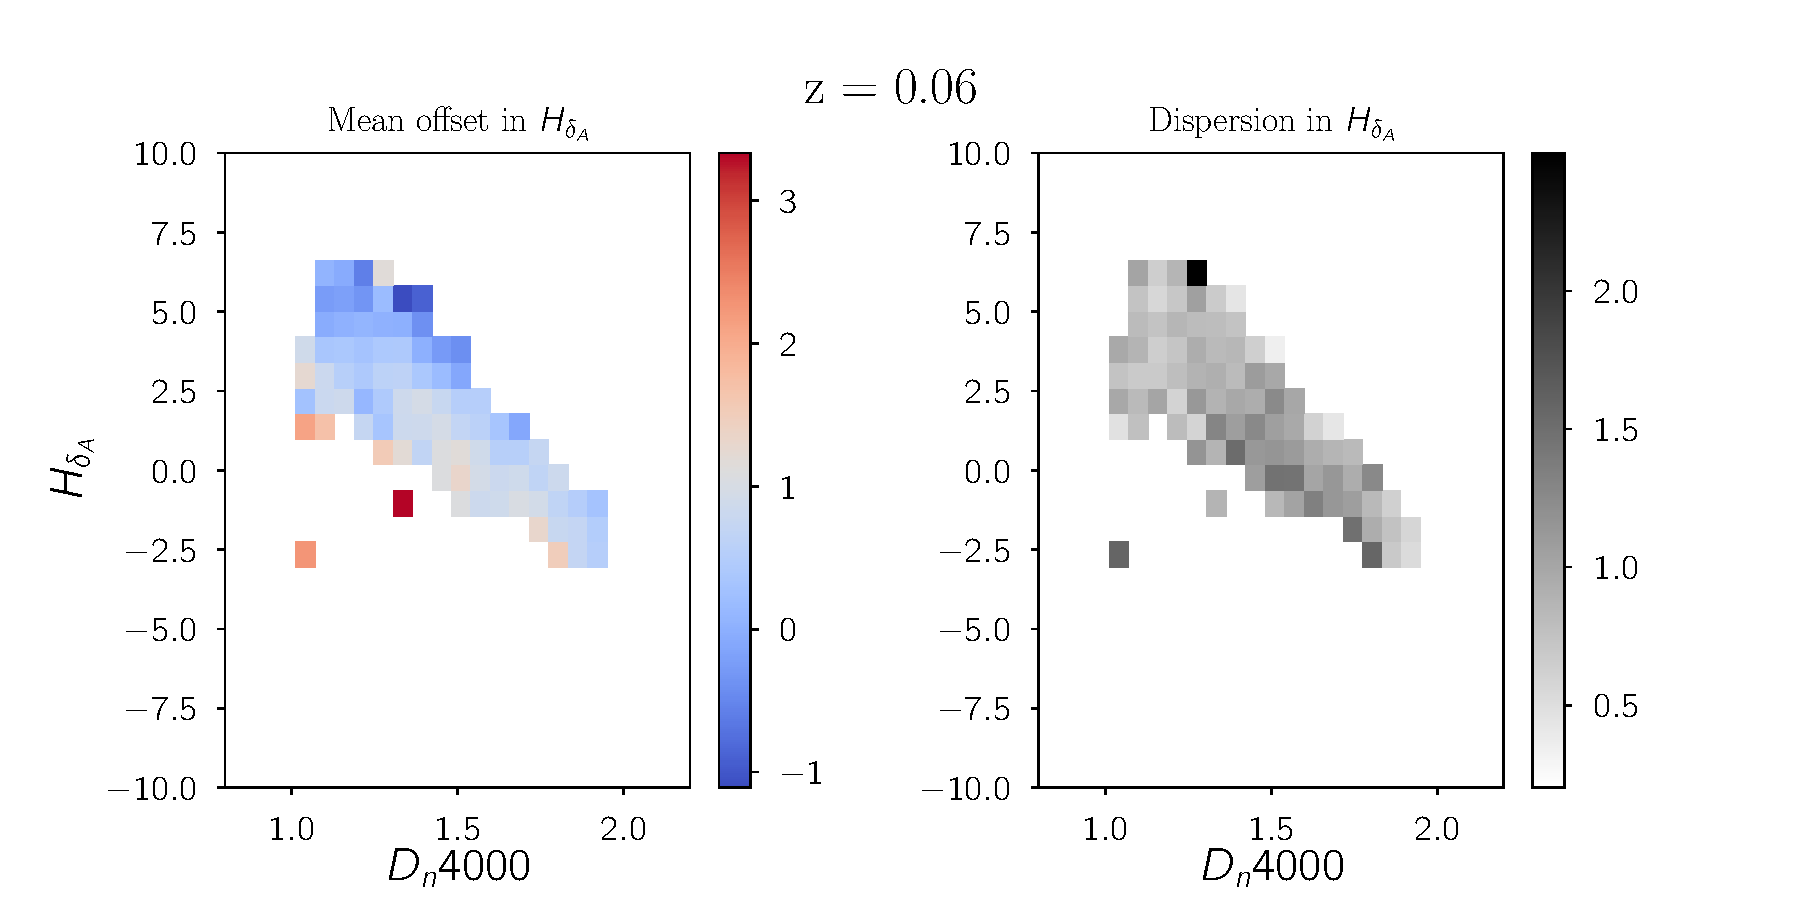
\includegraphics[width=\textwidth]{figures/z6c.pdf}
\caption[Short figure name.]{ The mean offset and dispersion in the $h\delta_{A}$ index measured at $z = 0.06$ with a $3$" aperture from the full aperture measurement 
\label{fig:myInlineFigure}}
\end{figure}

\begin{figure}
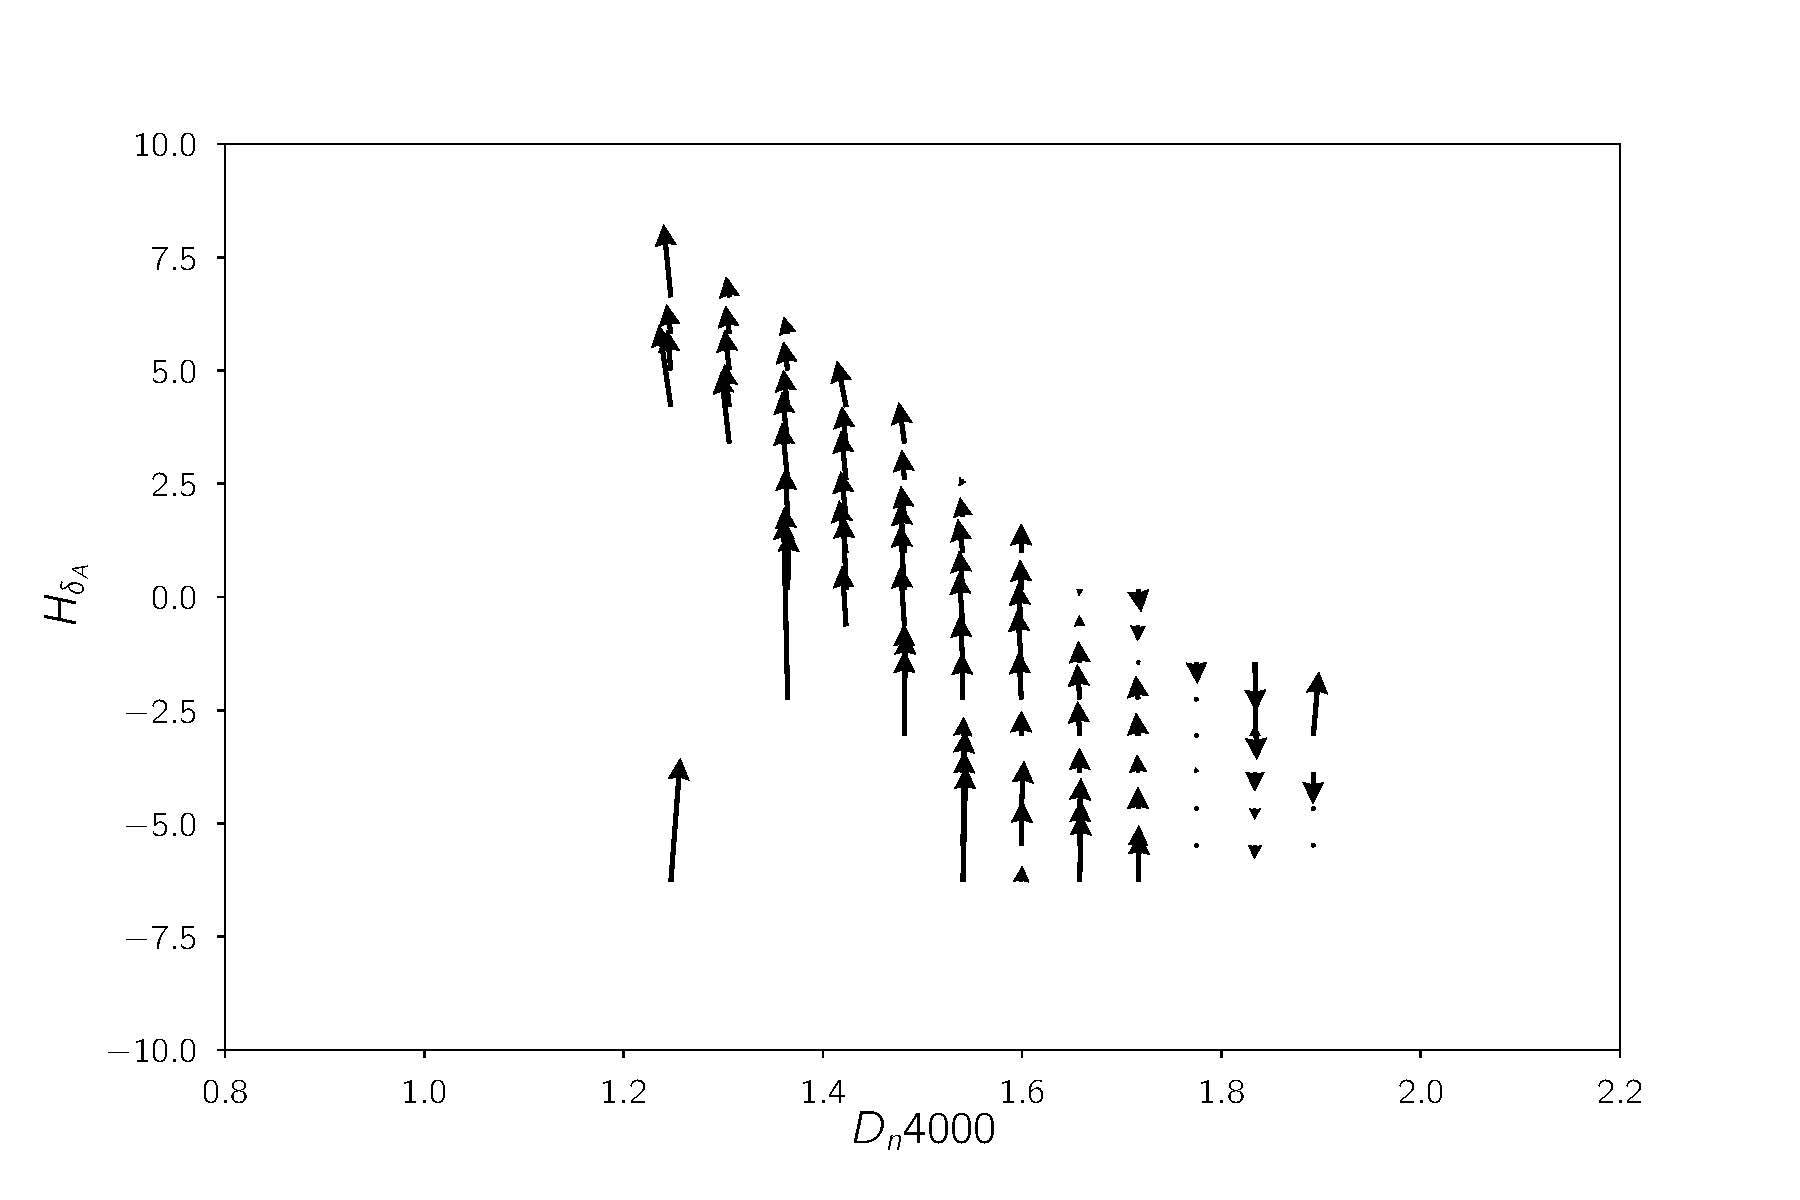
\includegraphics[width=\textwidth]{figures/z6d.pdf}
\caption[Short figure name.]{ The mean offset at $z=0.06$ plotted as a vector in the $D_{n}4000$, $h\delta_{A}$ plane
\label{fig:myInlineFigure}}
\end{figure}


